\documentclass{article}

\usepackage{amsmath}
\usepackage{amssymb}
\usepackage{mathpartir}
\usepackage{fontawesome5}
\usepackage{xcolor}
\usepackage{tikz}
\usetikzlibrary{arrows.meta,positioning}
\tikzset{graphnode/.style={draw,circle,inner sep=1.5pt,minimum size=18pt}}
\mprset{flushleft}

\newcommand{\kw}[1]{\text{\textbf{#1}}}
\newcommand{\judge}[3]{#1 \vdash #2 : #3}
\newcommand{\Jud}[2]{\judge{\Gamma}{#1}{#2}}
\newcommand{\leqto}{\mathrel{\leq_{\mathrm{to}}}}
\newcommand{\leqin}{\mathrel{\leq_{\mathrm{in}}}}
\newcommand{\mode}[1]{\textsc{#1}}
\newcommand{\subtype}{\mathrel{\sqsubseteq}}
\newcommand{\Alias}[2]{#1 \mathrel{\underset{\text{alias}}{\rightsquigarrow}} #2}
\newcommand{\Lock}[2][]{\text{\faLock}_{#1}(#2)}

\newcommand{\Rel}[2]{\mathcal{R}_{#1}(#2)}
\newcommand{\Solve}[1]{\mathsf{solve}(#1)}
\newcommand{\Constraint}[1]{\mathcal{C}\!\left(#1\right)}

\newcommand{\todo}[1]{\textcolor{red}{\textbf{TODO:} #1}}

\title{Relational Solver Notes}
\author{Jules Jacobs}
\date{\today}

\begin{document}

\maketitle

\section{Roadmap}

This document sketches the relational solver that accompanies the Mox type system notes.
The goal is to develop a mode solver that is powerful enough to handle the mode constraints produced by the type checker.

At a high level, we will develop a solver for binary constraints between modes.
We will first analyze a class of constraints that can be solved in polynomial time.
Then we will develop a more powerful solver that can handle that class of constraints.

\section{Constraint Language}

As a first step, assume we have a finite domain $V$ of values, and a set of binary relations $R_i \subseteq V \times V$.
Given a set of variables and asserted contraints between them, we want to determine if there exists a valuation of the variables that satisfies all the constraints.

In general this is a NP-complete problem: consider $V=\{0,1,2,\dots,k\}$ and $R_1 = \{ (a,b) \mid a \neq b \} \subseteq V \times V$.
Given a graph we can use this constraints to encode the $k$-coloring problem: we want to assign a color to each vertex such that no two adjacent vertices have the same color. The $k$-coloring problem is NP-complete, so this problem is also NP-complete.

However, certain classes of constraints can be solved in polynomial time. Consider the set of constraints $R_i = \{ (a,b) \mid b \geq a + i \} \subseteq V \times V$. Given a graph of variables and constraints, we can solve this problem in polynomial time using the Floyd-Warshall algorithm.

Equivalently, we can solve the problem by variable elimination: we take a variable $x$ and all adjacent constraints on it. We assert all transitive constraints (where $R_i$ composes with $R_j$ to produce $R_{i+j}$) and repeat until all variables are eliminated.
If, during this process, we ever see a constraint between a variable and itself with $i \neq 0$, then the constraints are unsatisfiable.

Why does this elimination strategy work for this class of constraints, but not for the general case, and in particular for the $k$-coloring problem with inequality constraints?

Consider a variable $x$ with:
\begin{itemize}
    \item a set of predecessors $a_1,a_2,a_3$ with $R_{i_1}(a_1,x), R_{i_2}(a_2,x), R_{i_3}(a_3,x)$ constraints on them,
    \item a set of successors $b_1,b_2$ with $R_{j_1}(x,b_1), R_{j_2}(x,b_2)$ constraints on them,
\end{itemize}
When eliminating $x$, we assert every transitive constraint $R_{i_p + j_q}(a_p,b_q)$ for $p \in \{1,2,3\}$ and $q \in \{1,2\}$:

\begin{figure}[ht]
  \centering
  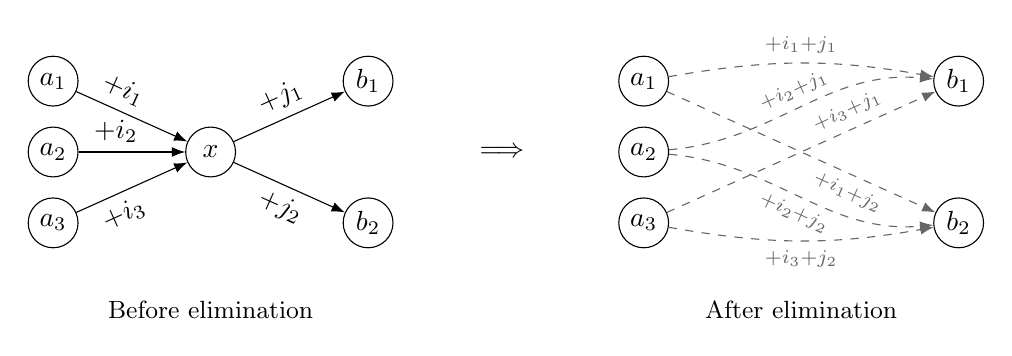
\begin{tikzpicture}[>=Latex]
    \begin{scope}[xshift=-2.5cm]
      \node[graphnode] (a1) at (0,0.9) {$a_1$};
      \node[graphnode] (a2) at (0,0) {$a_2$};
      \node[graphnode] (a3) at (0,-0.9) {$a_3$};
      \node[graphnode] (x)  at (2,0) {$x$};
      \node[graphnode] (b1) at (4,0.9) {$b_1$};
      \node[graphnode] (b2) at (4,-0.9) {$b_2$};

      \draw[->] (a1) -- node[pos=0.35,above,sloped] {$+i_1$} (x);
      \draw[->] (a2) -- node[pos=0.35,above] {$+i_2$} (x);
      \draw[->] (a3) -- node[pos=0.35,below,sloped] {$+i_3$} (x);

      \draw[->] (x) -- node[above,sloped] {$+j_1$} (b1);
      \draw[->] (x) -- node[below,sloped] {$+j_2$} (b2);

      \node[font=\small,align=center] at (2,-2) {Before elimination};
    \end{scope}

    \node at (3.2,0) {$\Longrightarrow$};

    \begin{scope}[xshift=5cm]
      \node[graphnode] (a1p) at (0,0.9) {$a_1$};
      \node[graphnode] (a2p) at (0,0) {$a_2$};
      \node[graphnode] (a3p) at (0,-0.9) {$a_3$};
      \node[graphnode] (b1p) at (4,0.9) {$b_1$};
      \node[graphnode] (b2p) at (4,-0.9) {$b_2$};

      \draw[dashed,->,black!60] (a1p) to[out=10,in=170] 
        node[pos=0.5,sloped,above,font=\scriptsize] {$+i_1{+}j_1$} (b1p);
      \draw[dashed,->,black!60] (a1p) --
        node[pos=0.7,sloped,below,font=\scriptsize] {$+i_1{+}j_2$} (b2p);

      \draw[dashed,->,black!60] (a2p) to[out=5,in=175]
        node[pos=0.5,sloped,above,font=\scriptsize] {$+i_2{+}j_1$} (b1p);
      \draw[dashed,->,black!60] (a2p) to[out=-5,in=-175]
        node[pos=0.5,sloped,below,font=\scriptsize] {$+i_2{+}j_2$} (b2p);

      \draw[dashed,->,black!60] (a3p) --
        node[pos=0.7,sloped,above,font=\scriptsize] {$+i_3{+}j_1$} (b1p);
      \draw[dashed,->,black!60] (a3p) to[out=-10,in=-170]
        node[pos=0.5,sloped,below,font=\scriptsize] {$+i_3{+}j_2$} (b2p);

      \node[font=\small,align=center] at (2,-2) {After elimination};
    \end{scope}
  \end{tikzpicture}
\end{figure}

I claim that if there is a solution for the neighboring variables that satisfies all of those transitive constraints, then there is a solution for $x$ that satisfies the original constraints: we can simply set $x$ to any value in the interval $\max(a_1 + i_1, a_2 + i_2, a_3 + i_3) \leq x \leq \min(b_1 + j_1, b_2 + j_2)$. This interval is guaranteed to be non-empty if the transitive constraints hold.

The key blocker for $k$-coloring is that this property does not hold for inequality constraints. Suppose for example we have a vertex $x$ and $k+1$ neighbors with inequality constraints. The transitive constraints are trivial if $k \geq 3$, because if we have $a \neq x \neq b$, then for a given value of $a$, all values of $b$ are still possible, by choosing a particular value for $x$. Thus, the strategy of variable elimination does not work for $k$-coloring, for $k \geq 3$: for $\neq$ constraints, eliminating $x$ produces no useful transitives; every neighbour pair remains unconstrained:

\begin{figure}[ht]
  \centering
  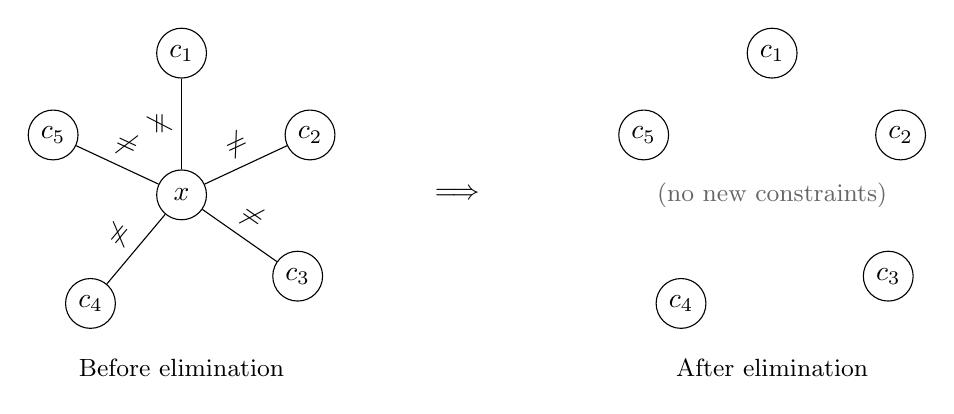
\begin{tikzpicture}[>=Latex]
    \begin{scope}[xshift=-2.5cm]
      \node[graphnode] (x2) at (0,0) {$x$};
      \foreach \angle/\name in {90/c_1,25/c_2,-35/c_3,-130/c_4,155/c_5} {
        \node[graphnode] (\name) at (\angle:1.8) {$\name$};
        \draw[-] (x2) -- node[midway,sloped,above] {$\neq$} (\name);
      }
      \node[font=\small,align=center] at (0,-2.2) {Before elimination};
    \end{scope}

    \node at (1,0) {$\Longrightarrow$};

    \begin{scope}[xshift=5cm]
      \node[graphnode,opacity=0] (x3) at (0,0) {$x$};
      \foreach \angle/\name in {90/c_1,25/c_2,-35/c_3,-130/c_4,155/c_5} {
        \node[graphnode] (\name p) at (\angle:1.8) {$\name$};
      }
      \node[font=\small,color=black!60] at (0,0) {(no new constraints)};
      \node[font=\small,align=center] at (0,-2.2) {After elimination};
    \end{scope}
  \end{tikzpicture}
\end{figure}

The OxCaml mode solver has constraints of the form $x \leq G(y)$ where $G$ are modalities with left adjoints. Like the interval constraints we considered above, these constraints can be solved in polynomial time using variable elimination, and for the same reason.

\subsection{Which constraints can be solved by elimination?}

For a set of constraints to be solvable by elimination, we need that the original problem has a solution iff the transformed problem has a solution. We will now analyze precisely when this property holds, and provide an easily checkable criterion for it.

\newcommand{\RelSet}{\mathsf{Rel}}
Let's first analyze the problem more precisely. Given a domain $V$ and a family of relations $\RelSet \subseteq \mathcal{P}(V \times V)$, the elimination algorithm may construct new relations in the following four ways:

\begin{itemize}
  \item It composes two relations $R,S \in \RelSet$ to produce $$RS = \{ (a,b) \mid \exists c.\ (a,c) \in R \land (c,b) \in S \}$$
  \item It intersects two relations $R,S \in \RelSet$ when it merges two parallel edges $$R \cap S = \{ (a,b) \mid (a,b) \in R \land (a,b) \in S \}$$
  \item It reverses the direction of a relation $R \in \RelSet$ to produce $$R^T = \{ (b,a) \mid (a,b) \in R \}$$
  \item We strengthen a relation $R \in \RelSet$ asserted between a variable and itself
  $$R^\ast = \{ (a,a) \mid (a,a) \in R \}$$
\end{itemize}

We therefore first close $\RelSet$ under these three operations. If the domain $V$ is finite, the resulting set of relations is finite.

Without loss of generality, we can picture the relations adjacent to a particular variable $x$ as follows:

\[
  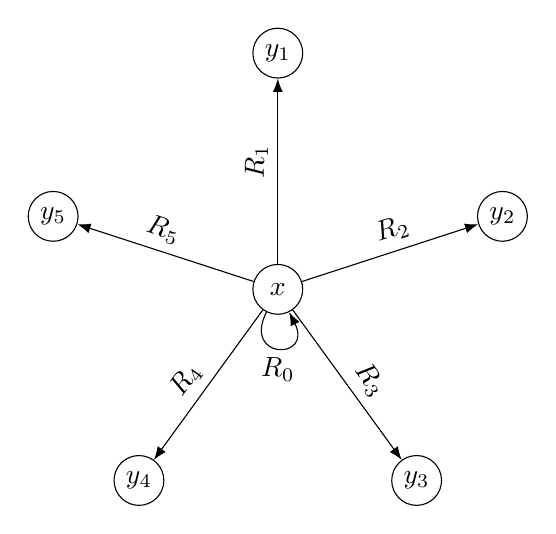
\begin{tikzpicture}[>=Latex]
    \node[graphnode] (xcore) at (0,0) {$x$};

    \foreach \idx/\angle in {1/90,2/18,3/-54,4/-126,5/162} {
      \node[graphnode] (y\idx) at (\angle:3) {$y_{\idx}$};
      \draw[->] (xcore) -- node[pos=0.55,above,sloped] {$R_{\idx}$} (y\idx);
    }

    \draw[->] (xcore) .. controls (-0.45,-0.9) and (0.45,-0.9) .. node[pos=0.5,below] {$R_{0}$} (xcore);
  \end{tikzpicture}
\]

\begin{figure}[ht]
  \centering
  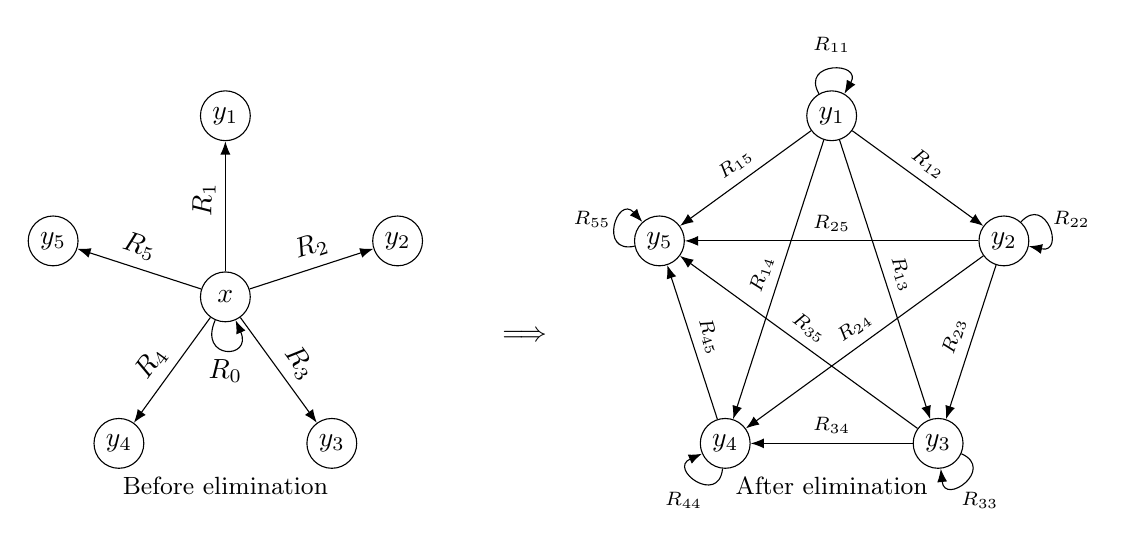
\begin{tikzpicture}[>=Latex]
    \begin{scope}[xshift=-3.5cm]
      \node[graphnode] (xbefore) at (0,0) {$x$};
      \foreach \idx/\angle in {1/90,2/18,3/-54,4/-126,5/162} {
        \node[graphnode] (yB\idx) at (\angle:2.3) {$y_{\idx}$};
        \draw[->] (xbefore) -- node[pos=0.55,above,sloped] {$R_{\idx}$} (yB\idx);
      }
      \draw[->] (xbefore) .. controls (-0.35,-0.8) and (0.35,-0.8) .. node[pos=0.5,below] {$R_{0}$} (xbefore);
      \node[font=\small] at (0,-2.4) {Before elimination};
    \end{scope}

    \node at (0.3,-0.5) {$\Longrightarrow$};

    \begin{scope}[xshift=4.2cm]
      \foreach \idx/\angle in {1/90,2/18,3/-54,4/-126,5/162} {
        \node[graphnode] (yA\idx) at (\angle:2.3) {$y_{\idx}$};
        \draw[->] (yA\idx) .. controls +({\angle+30}:0.8) and +({\angle-30}:0.8) .. (yA\idx);
        \path (yA\idx) ++({\angle}:0.9) node[font=\scriptsize] {$R_{\idx\idx}$};
      }

      \foreach \i/\j in {5/4,5/3,5/2,5/1,4/3,4/2,4/1,3/2,3/1,2/1} {
        \draw[->] (yA\j) -- node[pos=0.5,above,font=\scriptsize,sloped] {$R_{\j\i}$} (yA\i);
      }

      \node[font=\small] at (0,-2.4) {After elimination};
    \end{scope}
  \end{tikzpicture}
  \caption{Eliminating $x$ in the radial layout yields edges $R_{ij} = R_{i}^{\top} R_{0}^{\ast} R_{j}$ directed from $y_j$ to $y_i$ for all $i \geq j$, including self-loops $R_{ii}$.}
\end{figure}

\section{Solver Architecture}

\section{Open Questions}

\end{document}
